\ifx\allfiles\undefined
\documentclass{XDBAthesis}
\def\pictures{}
\begin{document}
\else
\fi
\chapter{图像处理及手势识别}

在手势识别中,处理的对象是手势的照片,我们提取数据的目标就是将手势的图像用一个特征向量来表示出来。在本文中所处理的图片主要有TIFF与BMP两种格式,TIFF格式相对来说要复杂一些,可以存储的图像也要丰富得多,它可以存储多张图片,还可以存储多种压缩格式的图片,而BMP格式的图片简单、通用,一般在应用程序中可以方便的显示。因此我们的工作除了熟悉多种格式的图像文件以外,还包括实现多种格式图像文件之间的相互转换,并最终提取出表示图像的特征向量。

\section{通用的图像操作}

    在手势识别中有很多常用的图像操作,例如图像的剪切、图像的缩放、图像的旋转以及图像的亮度调整。我们以\emph{Pixe1Array[x,y]}来表示原有图像的二维像素矩阵,原有图像的高度用H来表示,原有图像的宽度用\emph{W}来表示,用\emph{PjxelArrayNew[x,y]}来表示结果图像的二维像素矩阵,结果图像的高度为\emph{HNew},宽度为\emph{WNew}。

\subsection{图像的剪切}

    图像的剪切操作的函数原型为\emph{void CImage::eliplmage(eReet\&reet)},需
要输入的参数为要剪切的图像的具体的位置,即要剪切图像左上角的位置和右下角的位置。

假定要剪切图像左上角位置为\emph{(left,top)},右下角的位置\emph{(right,bottom)},那我们只需要调整图像的宽度为\emph{(righi-left)},调整图像的高度\emph{(bottom-top)},从图像的二维数组中提取左上角到右下角之间的数据。剪切后图像的数据可以表示为:



\subsection{图像的缩放}

    图像的缩放操作的函数原型为\emph{void CImage::CollapseOrExpandlmage(double dbRatioX,double dbRatioY)}。输入的参数为图像水平方向需要缩放的尺度以及图像垂直方向需要缩放的尺度。

假定水平方向缩放的比例为\emph{a},垂直方向缩放的比例为\emph{b},那么,缩放后图像的高度为\emph{bH},缩放后图像的宽度为\emph{aw},对于原有图像的任一点\emph{PixelArray[x,y]},在缩放后对应的像素为:



    令\emph{CountArray[i,j]}为结果图像中点\emph{(i,j)}对应原有图像像素的计数,那么每次有点映射到点\emph{(i,j)}的像素时,将结果图像中点\emph{(i,j)}的像素值加上该原有图像点\emph{(x,y)}的像素值,并将\emph{CountArray[i,j]}加l。

由于经缩放后,结果图像中的某一点的像素可能对应原有图像中的多个像素,所以对于这种情况需要对该点的像素求取平均值:



    图像缩放操作可以用一个简单的示意图(图\ref{fg:ss})来表示:
    
\begin{figure}[htb]
    \centering
    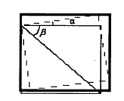
\includegraphics[width=0.5\textwidth]{figure/roat}
    \caption{缩放示意图}
    \label{fg:ss}
\end{figure}

\subsection{图像的旋转}

    图像的旋转在所有的通用操作中是最复杂的,它的函数原型为\emph{void CImage::Rotatelmage(double dbAngle)}。从中可以看出,传入的参数是需要旋转的角度,该角度以弧度值来表示,正数表示的是逆时针方向旋转,负数表示的是顺时针方向旋转。

旋转操作的示意图如图\ref{fg:roat}所示(逆时针旋转\emph{Q}度):
\begin{figure}[htb]
    \centering
    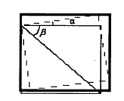
\includegraphics[width=0.5\textwidth]{figure/roat}
    \caption{旋转示意图}
    \label{fg:roat}
\end{figure}
      

图中细黑色的表示原来图像的范围,粗黑色的为旋转后图像的范围,虚线的为原来图像经旋转后在结果图像中的位置。

旋转操作首先需要判断该角度属于哪一个象限,不同的象限所使用的变换公式是不同的。假定输入的旋转角度为,令已为口经变换后在\emph{[0,]}之间的角度,令为经变换后在之间的角度,其中:


这样在任意的旋转角度下,原图像中的每一点都可以对应到新图像中的某一点中,考虑到经过旋转后在新图像中对应原图像部分的内部可能存在某些点在原图像中不存在对应点,所以需要对这些点作平滑处理,使图像达到连续的效果。

\section{手势图像预处理}

\subsection{灰度处理}

在进行视频流目标识别与跟踪时,通常第一个步骤就是对采集到的彩色图像进行灰度化,这是因为黑白照片数据量小,相比彩照更易实现实时算法,另一方面黑白照片是由未处理的光线所形成的照片,因此从图像处理学角度来看,这种未经特殊滤光处理的图片所涵盖的信息更有价值。

由于在OpenCV中自带函数可以实现图像灰度化,因此在该问题处理中直接调用函数\emph{:cvCreateImage}。实现过程如图\ref{fg:hui}。

 \begin{figure}[htb]
    \centering
    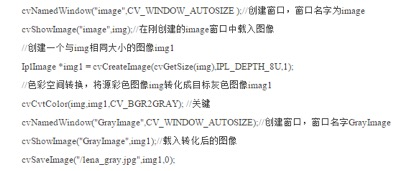
\includegraphics[width=\textwidth]{figure/hui}
    \caption{灰度处理实现代码}
    \label{fg:hui}
\end{figure}

\subsection{平滑处理}

消除图像中随机噪声的技术。对平滑技术的基本要求是在消去噪声的同时不使图像轮廓或线条变得模糊不清。常用的平滑方法有中值法、局部求平均法和k 近邻平均法。局部区域大小可以是固定的,也可以是逐点随灰度值大小变化的。此外,有时应用空间频率域带通滤波方法。

对于平滑处理,在OpenCV函数库中也有相应的函数:

\emph{CV\_BLUR\_NO\_SCALE} (简单不带尺度变换的模糊) - 对每个象素的 $param1\times param2$ 领域求和。如果邻域大小是变化的,可以事先利用函数 \emph{cvIntegral} 计算积分图像。

\emph{CV\_BLUR} (simple blur) - 对每个象素$param1\times param2$邻域 求和并做尺度变换 $1/(param1\times param2)$。

\emph{CV\_GAUSSIAN} (gaussian blur) - 对图像进行核大小为 $param1\times param2$ 的高斯卷积。

\emph{CV\_MEDIAN} (median blur) - 对图像进行核大小为$param1\times param1$ 的中值滤波 (i.e. 邻域是方的)。

\emph{CV\_BILATERAL} (双向滤波) - 应用双向 $3\times 3$ 滤波,彩色 $sigma=param1$,空间 $sigma=param2$。param1平滑操作的第一个参数。param2平滑操作的第二个参数。对于简单/非尺度变换的高斯模糊的情况,如果param2的值为零,则表示其被设定为param1。

\section{手势特征提取}

    特征提取是计算机视觉和图像处理中的一个概念。它指的是使用计算机提取图像信息,决定每个图像的点是否属于一个图像特征。特征提取的结果是把图像上的点分为不同的子集,这些子集往往属于孤立的点、连续的曲线或者连续的区域。

特征提取与选择一般分为三个步骤:特征形成、特征提取、特征选择。

特征形成  有信号获取或测量得到原始测量,之后处理后得到图像特征,这样的特征称作原始特征,如手势图像属于数字图像,它的原始测量是各点灰度值,但是这些测量不适于作为特征,还要经过计算产生一组原始特征。

     特征提取  原始特征的数量可能很大,或者说样本是处于一个多维空间中,通过映射(变换)将原始特征变换为较少的新特征,这个过程称作特征提取。映射后的特征又称作二次特征,它们是原始特征的某种组合,所以特征提取在广义上就是一种特征映射。如公式\eqref{eq:tt}所示。
\begin{equation}
    A:Y\rightarrow X
    \label{eq:tt}
\end{equation}

其中\emph{Y}是测量空间,\emph{X}是特征空间,\emph{A}称为特征映射,又称作特征提取器。

     特征选择  从原始特征中挑出一些最具有代表性和分类性最好的特征,这个过程称为特征选择,它可以起到降低特征空间维数的作用。

\subsection{Canny检测轮廓}

Canny边缘检测器利用Canny算子进行检测,是目前最精确的检测器,并且已经被大量运用于程序中。从目前看来,canny边缘检测在做图像轮廓提取 方面是最优秀的边缘检测算法。

canny边缘检测采用双阈值值法,高阈值用来检测图像中重要的、显著的线条、轮廓等,而低阈值用来保证不丢失细节部分,低阈值检测出来的边缘更丰富,但是很多边缘并不是我们关心的。最后采用一种查找算法,将低阈值中与高阈值的边缘有重叠的线条保留,其他的线条都删除。

函数如下:

效果展示:



\subsection{直线检测}

直线在图像中出现的频率非常之高,而直线作为图像的特征对于基本内容的图像分析有着很重要的作用,我们通常通过OpenCV中的hough变换来检测图像中的线条。

首先展示最基本的Hough变换函数HoughLines,它的原型如图\ref{fg:yuan} 所示。
\begin{figure}[htb]
    \centering
    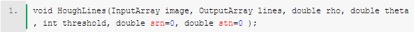
\includegraphics[width=\textwidth]{figure/code}
    \caption{HoughLines原型}
    \label{fg:yuan}
\end{figure}

 

    它的输入是一个二值的轮廓图像,往往是边缘检测得到的结果图像;它的输出是一个包含多个\emph{Vec2f}点的数组,数组中的每个元素是一个二元浮点数据对\emph{<rou,theta>}而言,\emph{rou}代表直线离坐标原点的距离,\emph{theta}代表角度。第3和第4个参数代表步长,因为\emph{Hough}变换实际上是一个穷举的算法,\emph{rho}表示距离的步长,\emph{theta}代表角度的步长。第5个参数是一个阈值设置直接的最低投票个数,知道\emph{Hough}原理的,这个参数应该很容易理解。

   从这个函数的输出结果我们可以看出,得到的直线并没有指定在图像中的开始点与结束点,需要我们自己去计算,如果我们想把直接显示在图像中就会比较麻烦,而且 会有很多角度接近的直线,其实它们是重复的,为了解决上面这些问题,\emph{OpenCV}又提供了一个函数\emph{HoughLinesP()}。它的输出是一个 \emph{Vector of Vec4i}。\emph{Vector}每一个元素代表一条直线,是由一个4元浮点数组构成,前两个点一组,后两个点一组,代表了在图像中直线的起始和结束点。

\subsection{轮廓的提取与描述}

在目标识别中,首先要把感兴趣的目标提取出来,而一般常见的步骤都是通过颜色或纹理提取出目标的前景图(一幅黑白图像,目标以白色显示在图像中),接下来要对前景图进行分析进一步地把目标提取出来,而这里常常用到的就是提取目标的轮廓。

OpenCV 里提取目标轮廓的函数是\emph{findContours},它的输入图像是一幅二值图像,输出的是每一个连通区域的轮廓点的集 合:\emph{vector<vector<Point>>}。外层\emph{vector}的\emph{size}代表了图像中轮廓的个数,里面\emph{vector}的\emph{size}代表了轮廓上点的个数。

提取到轮廓后,最重要的就是如何把这些轮廓转换为可以利用的特征,也就是涉及到轮廓的描述问题,这时就有多种方法可以选择,比如矢量化为多边形、矩形、椭圆等。OpenCV里提供了一些相应函数,在这里就不详细介绍了。  


\ifx\allfiles\undefined
%\bibliographystyle{unsrt}
\bibliography{main}
\end{document}
\fi